\documentclass{article}

\usepackage{amsmath, amsfonts, amsthm} % Math packages

\usepackage{listings} % Code listings, with syntax highlighting

\usepackage[main = greek, english]{babel} % English language hyphenation

\usepackage{graphicx} % Required for inserting images
\graphicspath{{Figures/}{./}} % Specifies where to look for included images (trailing slash required)

\usepackage{booktabs} % Required for better horizontal rules in tables

\usepackage{dirtytalk} % Required for quoting.

\usepackage{float} % Added for hard placement of images.

\usepackage[dvipsnames]{xcolor} % Added for extra colors.

\usepackage{tikz} % For colored boxes and more.

\numberwithin{equation}{section} % Number equations within sections (i.e. 1.1, 1.2, 2.1, 2.2 instead of 1, 2, 3, 4)
\numberwithin{figure}{section} % Number figures within sections (i.e. 1.1, 1.2, 2.1, 2.2 instead of 1, 2, 3, 4)
\numberwithin{table}{section} % Number tables within sections (i.e. 1.1, 1.2, 2.1, 2.2 instead of 1, 2, 3, 4)

\usepackage[utf8]{inputenc} % Required for inputting international characters
\usepackage[T1]{fontenc} % Use 8-bit encoding

\usepackage{translator}

\newcommand{\en}[1]{\foreignlanguage{english}{#1}}
\newcommand{\src}[1]{{\texttt\en{#1}}}


% Extra Formatting

\setlength{\parindent}{0em}
\setlength{\parskip}{0em}


% Code Listing Style

\lstdefinestyle{code}{
  belowcaptionskip=1\baselineskip,
  breaklines=true,
  frame=LRTB,
  xleftmargin=\parindent,
  showstringspaces=false,
  basicstyle=\ttfamily,
  keywordstyle=\bfseries\color{green!40!black},
  commentstyle=\itshape\color{purple!40!black},
  identifierstyle=\color{black},
  stringstyle=\color{orange},
}


\newcommand{\lstcode}[3]
{
    \begin{otherlanguage}{english}
    \lstinputlisting[language=#2, frame=single, style=code, caption=#3]{#1}
    \end{otherlanguage}
}

\usepackage{lineno}
\usepackage{hyperref}
\usepackage{cleveref}
\usepackage{epigraph} 
\modulolinenumbers[5]

\usetikzlibrary{positioning}
\usetikzlibrary{dsp,chains}

\DeclareMathAlphabet{\mathpzc}{OT1}{pzc}{m}{it}
\newcommand{\z}{\mathpzc{z}}

\crefname{equation}{εξ.}{εξ.}
\crefname{listing}{καταχώριση}{καταχώριση}

\makeindex

\bibliographystyle{ieeetr}

\begin{document}

\begin{titlepage}

\title{Σχεδιασμός και υλοποίηση ψηφιακού ισοσταθμιστή ήχου.}
% \tnotetext[mytitlenote]{Fully documented templates are available in the elsarticle package on \href{http://www.ctan.org/tex-archive/macros/latex/contrib/elsarticle}{CTAN}.}

%% Group authors per affiliation:
\author{Ευάγγελος Λάμπρου}
\date{}

\maketitle

\begin{abstract}
    Στα πλαίσια αυτής της εργασίας γίνεται ο σχεδιασμός και υλοποίηση 
    ενός ισοσταθμιστή ήχου. 
    Η ανάπτυξή του συστήματος ψηφιακής επεξεργασίας σήματος, όπως 
    και η γραφική διεπαφή έγιναν μέσα στο περιβάλλον του 
    \en{JUCE Framework} χρησιμοποιώντας τη γλώσσα \en{C++}. 
    Στην εργασία αυτή γίνεται η ανάλυση της θεωρίας πίσω από την ανάπτυξη των φίλτρων, 
    την υλοποίηση του συστήματος από το χαμηλό έως το υψηλό επίπεδο αφαιρετικότητας που 
    προσφέρει το πακέτο \en{JUCE}. 
    Τέλος, υπάρχει ανάλυση των επιδόσεων του φίλτρου όπως και μία σύντομη αναφορά πάνω 
    στην ευκολία χρήσης του.
\end{abstract}


\end{titlepage}

\linenumbers

\section{Σχεδιασμός}

\begin{figure}[htpb]

    \begin{center}

        \begin{tikzpicture}

        % Controller

        \node [draw,
        fill=Goldenrod,
        minimum width=2cm,
        minimum height=1.2cm,
        right=1cm
            ] (dsp) {$DSP$};

        \draw[->] ++(-1,0) -- (dsp.west) 
            node[midway,above]{$audio_{in}$};

        \draw[->] ++(-1,0) -- (dsp.west) 
            node[midway,above]{$audio_{in}$};

        \draw[->] (dsp.east) --  ++(+2,0) 
            node[midway,above]{$audio_{out}$};
        \end{tikzpicture}
    \end{center}

    \caption{Βασική δομή του \en{plugin}.} 
\end{figure}

\paragraph{Θεωρία \en{IIR} φίλτρων}

Στην εργασία αυτή θα περιοριστούμε στην υλοποίηση φίλτρων 2ης τάξης, με τους 
αλγόριθμους όμως να είναι ικανούς να παράγουν φίλτρα οσοδήποτε μεγάλης τάξης (χωρίς 
βέβαια να εγγυάται η ορθότητα του τελικού αποτελέσματος λόγω πεπαρασμένης ακρίβειας 
στις τιμές των συντελεστών). 

Έχοντας ως βάση ένα χαμηλοπερατό φίλτρο 2ης τάξης \cite{OpenheimAlan}

\begin{equation}
    H(s) = \frac{1}{s^2 + s/Q + 1} 
    \label{eq:h_lowpassfilter}
\end{equation}

Μέσω του διπολικού $Z$ μετασχηματισμού, θέτωντας $s = \frac{1}{K}\frac{z-1}{z+1} \; K = \frac{1}{2F_s}$ έχουμε \cite{BilinearZTransformWeb}

\begin{equation}
    H(z) = \frac{K^2 + 2K^2 z^{-1} + K^2 z^{-2}}{(K^2 + K/Q + 1) + 2(K^2 - 1) z^{-1} + (K^2 - K/Q + 1) z^{-2}}
    \label{eq:h_z_final}
\end{equation}


\paragraph{Φίλτρα \en{Butteworth}} 

Για τους συντελεστές του φίλτρου \en{Butterworth} μπορούμε απλά να υπολογίσουμε την τιμή 
της σταθεράς $Q$ και να πάρουμε τους συντελεστές από την \cref{eq:h_lowpassfilter} \cite{OpenheimAlan, JuceDocumentation}

\begin{align}
    1/Q &= {2cos(\frac{2i + 1}{n}\pi)}, \; i = 0..\frac{n}{2} \qquad n = {\text{άρτιο}} \\ 
    1/Q &= {2cos(\frac{i + 1}{2n}\pi)}, \; i = 0..\frac{n}{2} \qquad n = {\text{περιττό}}
\end{align}

\paragraph{Αλγόριθμος Υπολογισμού Συντελεστών}

Από την προηγούμενη μαθηματική ανάλυση, ο υπολογισμός των συντελεστών για το εκάστοτε φίλτρο είναι πλέον 
τετριμένος. 

Αντικαθιστώντας τις τιμές για το $Q$ για ένα φίτλρο \en{Butteworth} στη σχέση \ref{eq:h_z_final}
έχουμε πλέον τους συντελεστές του φίλτρου. 


\begin{align}
    a_0 &= \frac{K^2}{K^2 + K/Q +1} & a_1 &= 2a_0 & a_2 &= a_0 \\
    b_0 &= 1 & b_1 &= \frac{2(K^2 - 1)}{K^2 + K/Q + 1} & b_2 &= \frac{K^2 - K/Q + 1}{K^2 + K/Q + 1}
\end{align}

\section{Υλοποίηση}

Για την υλοποίηση του φίλτρου χρησιμοποιήθηκαν οι βιβλιοθήκες του πακέτου 
\en{Juce}. Το πακέτο αυτό χωρίζεται σε ενότητες \en{(modules)}, από τις οποίες
χρησιμοποιούμε κατά βάση την ενότητα \src{juce::dsp}. 
Εδώ, περιλαμβάνονται κλάσεις μέσω την οποίων μπορεί να γίνει η δημιουργία 
ενός φίλτρου.

Ο τρόπος με τον οποίο η εφαρμογή μας επεξεργάζεται τα εισερχόμενα δείγματα
\en{(samples)} είναι στη ρουτίνα \src{processBlock} όπου δεχόμαστε σαν είσοδο έναν
\en{buffer} από δείγματα στα οποία μπορούσαμε να εφαρφμόσουμε οποιονδήποτε αλγόριθμο. 

Το \en{plugin} στην πραγματικότητα αποτελείται από τρία (3) φίλτρα: 

\begin{enumerate}
    \item Ένα χαμηλοπερατό φίλτρο \en{(low pass filter)}
    \item Ένα φίλτρο κορυφής
    \item Ένα υψηπερατό φίλτρο
\end{enumerate}

Ο τρόπος με τον οποίο αυτό περιγράφεται στον κώδικα είναι μέσω της δομής 
\src{ProcessorChain} η οποία αναπαριστά μία αλυσιδά επεξεργαστών. 
Κατά την εκτέλεση της εφαρμογής, η ακολουθία από δείγματα
περνάει από την ρουτίνα επεξεργασίας του κάθε φίλτρου διαδοχικά. \cite{JuceDocumentation}

Ο υπολογισμός της νέας αριθμητικής τιμής του κάθε δείγματος γίνεται με 
τη σειρά που φαίνεται στη \cref{fig:iir_filter_block}. 
Η καθυστέρηση του σήματος εισόδου γίνεται εφόσων το \en{plugin}
αποθηκεύει την κατάστασή του, η οποία είναι ένας πίνακας με τις τιμές της εξόδου 
του στα προηγούμενα δείγματα. Στην περίπτωση ενός φίλτρου 2ης τάξης 
αρκεί να αποθηκεύουμε τις δύο (2) προηγούμενες τιμές εξόδου του.

Η υλόποιση σε κώδικα όπως φαίνεται στην \cref{lst:iirimp} ταυτίζεται με τη σχηματική 
αναπαράσταση. Η βιβλιοθήκη \src{JUCE} έχει προνοήσει για τη χρήση τον ρουτίνων 
της με αριθμητικούς τύπους διαφορετικής ακρίβειας, εξού και η άπλετη χρήση της 
λέξης-κλειδί \src{auto} \cite{CppReferenceAuto}, η οποία αναθέτει στον \en{compiler} το συμπέρασμα του τύπου 
της εκάστοτε μεταβλητής.

\vspace{5mm}

\begin{figure}
\centering
    \begin{tikzpicture}

	% Place nodes using a matrix
    \matrix (m1) [row sep=5mm, column sep=9mm]
    {
        \node[dspnodeopen, dsp/label=above] (x) {$x[n]$}     ; &
		\node[dspnodefull]                 (m11) {}          ; &
        \node[dspmixer, dsp/label=above]    (b0) {$b_0$}     ; &
        \node[dspadder]                     (adder) {}       ; &
		\node[coordinate]                   (m12) {}         ; &
		\node[dspnodefull]                   (m13) {}        ; &
        \node[dspnodeopen, dsp/label=above] (y) {$y[n]$}     ; &
        \\
        \node[coordinate]                   (mc) {}          ; &
		\node[dspsquare]                   (z01) {$\z^{-1}$} ; &
        \node[coordinate]                   (mc) {}          ; &
        \node[coordinate]                   (mc) {}          ; &
        \node[coordinate]                   (mc) {}          ; &
		\node[dspsquare]                   (z02) {$\z^{-1}$} ; &
        \\
        \node[coordinate]                   (mc) {}          ; &
        \node[dspnodefull]                   (m31) {}        ; &
        \node[dspmixer, dsp/label=above]    (b1) {$b_1$}     ; &
        \node[coordinate]                   (mc) {}          ; &
        \node[dspmixer, dsp/label=above]    (a1) {$-a_1$}    ; &
        \node[dspnodefull]                   (m32) {}        ; &
        \\
        \node[coordinate]                   (mc) {}          ; &
		\node[dspsquare]                   (z11) {$\z^{-1}$} ; &
        \node[coordinate]                   (mc) {}          ; &
        \node[coordinate]                   (mc) {}          ; &
        \node[coordinate]                   (mc) {}          ; &
		\node[dspsquare]                   (z12) {$\z^{-1}$} ; &
        \\
        \node[coordinate]                   (mc) {}          ; &
        \node[dspnodefull]                   (m51) {}        ; &
        \node[dspmixer, dsp/label=above]    (b2) {$b_2$}     ; &
        \node[coordinate]                   (mc) {}          ; &
        \node[dspmixer, dsp/label=above]    (a2) {$-a_2$}    ; &
        \node[dspnodefull]                   (m52) {}        ; &
        \\
    }                                                        ;

	% Draw connections

	\begin{scope}[start chain]
		\chainin (x);
		\chainin (m11) [join=by dspline];
		\chainin (b0) [join=by dspline];
		\chainin (adder) [join=by dspconn];
		\chainin (m13) [join=by dspconn];
		\chainin (y) [join=by dspconn];
	\end{scope}

	\begin{scope}[start chain]
		\chainin (m11);
		\chainin (z01) [join=by dspconn];
		\chainin (m31) [join=by dspconn];
		\chainin (b1) [join=by dspconn];
		\chainin (adder) [join=by dspconn];
	\end{scope}

	\begin{scope}[start chain]
		\chainin (m31);
		\chainin (z11) [join=by dspconn];
		\chainin (m51) [join=by dspconn];
		\chainin (b2) [join=by dspconn];
		\chainin (adder) [join=by dspconn];
	\end{scope}

	\begin{scope}[start chain]
		\chainin (m13);
		\chainin (z02) [join=by dspconn];
		\chainin (m32) [join=by dspconn];
		\chainin (a1) [join=by dspconn];
		\chainin (adder) [join=by dspconn];
	\end{scope}

	\begin{scope}[start chain]
		\chainin (m32);
		\chainin (z12) [join=by dspconn];
		\chainin (m52) [join=by dspconn];
		\chainin (a2) [join=by dspconn];
		\chainin (adder) [join=by dspconn];
	\end{scope}
	
\end{tikzpicture}


\caption{Υλοποίηση του \en{IIR} φίλτρου}
\label{fig:iir_filter_block}

\end{figure}

\begin{minipage}{\textwidth}
    \lstcode[lst:iirimp]{./assets/src/iir.cpp}{C++}{Ο υπολογισμός της νέας τιμής για το κάθε δείγμα σε \src{C++}}
\end{minipage}


\paragraph{Γραφική Διεπαφή}

\epigraph{\en{The first 90 percent of the code accounts for the first 90 percent of
the development time. The remaining 10 percent of the code accounts for the
other 90 percent of the development time}}{\en{\textit{Tom Cargill, Bell Labs}}}

Η βιβλιοθήκη \en{JUCE} παρέχει τη δυνανότητα να αναπτύξει ο χρήστης 
σύνθετες γραφικές διεπαφές μέσα από τις οποίες μπορεί κάποιος να ελέγχει 
το \en{DSP} μέρος της εφαρμογής (συχνότητες αποκοπής κτλ).

\begin{figure}[htpb]
    \centering
    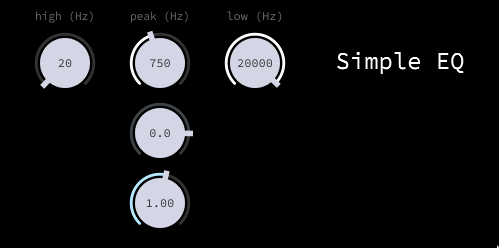
\includegraphics[width=0.8\textwidth]{./assets/GUI.png}
    \caption{Η τελική γραφική διεπαφή του ισοσταθμιστή.}
    \label{fig:finalgui}
\end{figure}

\paragraph{Χρήση}

\begin{figure}[htpb]
    \centering
    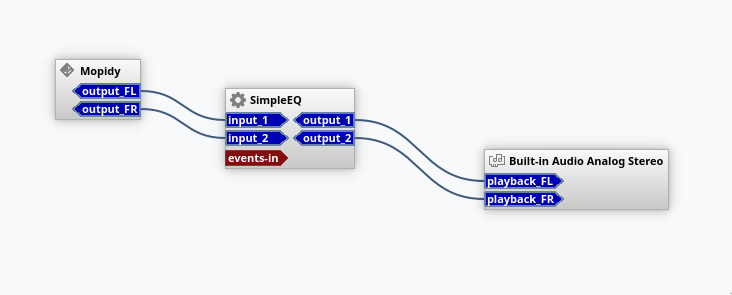
\includegraphics[width=0.8\textwidth]{./assets/Carla_Basic.png}
    \caption{Εφαρμογή του \src{SimpleEq plugin} στο περιβάλλον \en{Carla}.}
    \label{fig:carla_basic}
\end{figure}

Για την χρήση του \en{plugin} \src{Simple EQ} μπορεί να γίνει 
σύνδεσή του με άλλες ροές ήχου στον υπολογιστή μέσω ενός \en{audio plugin host}.
Ένα πολύ ικανό και δημοφιλές είναι το λογισμικό \en{Carla} \cite{CarlaApp}, 
μέσα από το οποίο μπορούμε να κατευθύνουμε τη ροή ήχου από μία εφαρμογή 
στον υπολογιστή μας, μέσα από κάποιο \en{plugin} και τελικά να έχουμε την έξοδο 
στα ηχεία (ή οποιαδήποτε άλλη συσκευή).

Πιο συνιθέστερη όμως θα είναι η χρήση του \en{plugin} μέσα από ένα λογισμικό 
\en{DAW (Digital Audio Workstation)}, όπου μπορούμε να φορτώσουμε δυναμικά 
το \src{Simple EQ}, να προσθέσουμε σε ένα από τα κομμάτια του \en{mixer} 
και έτσι όποιος ήχος περνάει σε εκείνο το κανάλι θα επεξεργάζεται από τον \en{plugin}. 

Η βιβιοθήκη \src{JUCE} προσφέρει συστήματα για το χτήσιμο του κώδικα 
ως \en{plugin (VST3)} \cite{VSTWiki}, ή ως αυτόνομη εφαρμογή.  

\paragraph{Μετρήσεις}

Μετά τη δημιουργία της εφαρμογής ισοστάθμισης, έγινε εισαγωγή του \en{plugin} 
\src{SimpleEQ} στο ψηφιακό περιβάλλον επεξεργασίας ήχου (\en{DAW}) \en{Ardour}, 
το οποίο λειτουργεί σαν υποδοχέας και παρέχει δυνατότητες μέτρησης της απόκρισης συχνότας και 
φάσης του φίλτρου (\cref{fig:ardour_analysis}).

\begin{figure}[htpb]
    \centering
    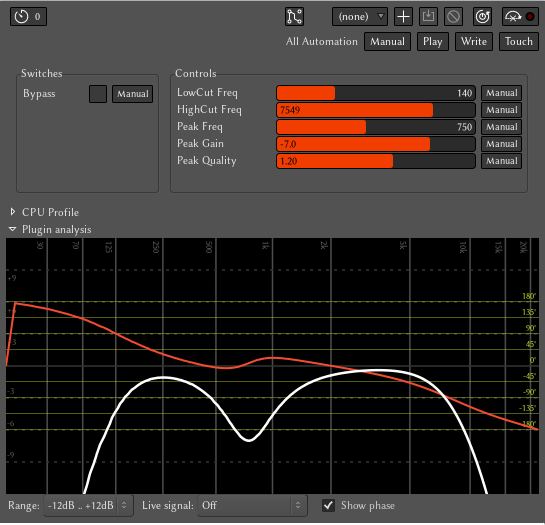
\includegraphics[width=0.8\textwidth]{./assets/PluginAnalysisArdour.png}
    \caption{Ανάλυση του \src{SimpleEQ} μέσα από το \en{Ardour}. Φαίνεται η απόκριση συχνότητας (άσπρο) και η απόκριση φάσης (κόκκινο).}
    \label{fig:ardour_analysis}
\end{figure}

Για μερικές ακόμα μετρήσεις χρησιμοποιήθηκε το τραγούδι \en{Bring Me the Disco King - David Bowie} 
το οποίο περάσαμε μέσα από \src{Simple EQ}. 

Όλα τα αρχεία τα οποία μελετάμε είναι κωδικοποιημένα σε μορφή \en{WAV 16-bit} με συχνότητα δειγματοληψίας $48kHz$.

\begin{figure}[htpb]
    \centering
    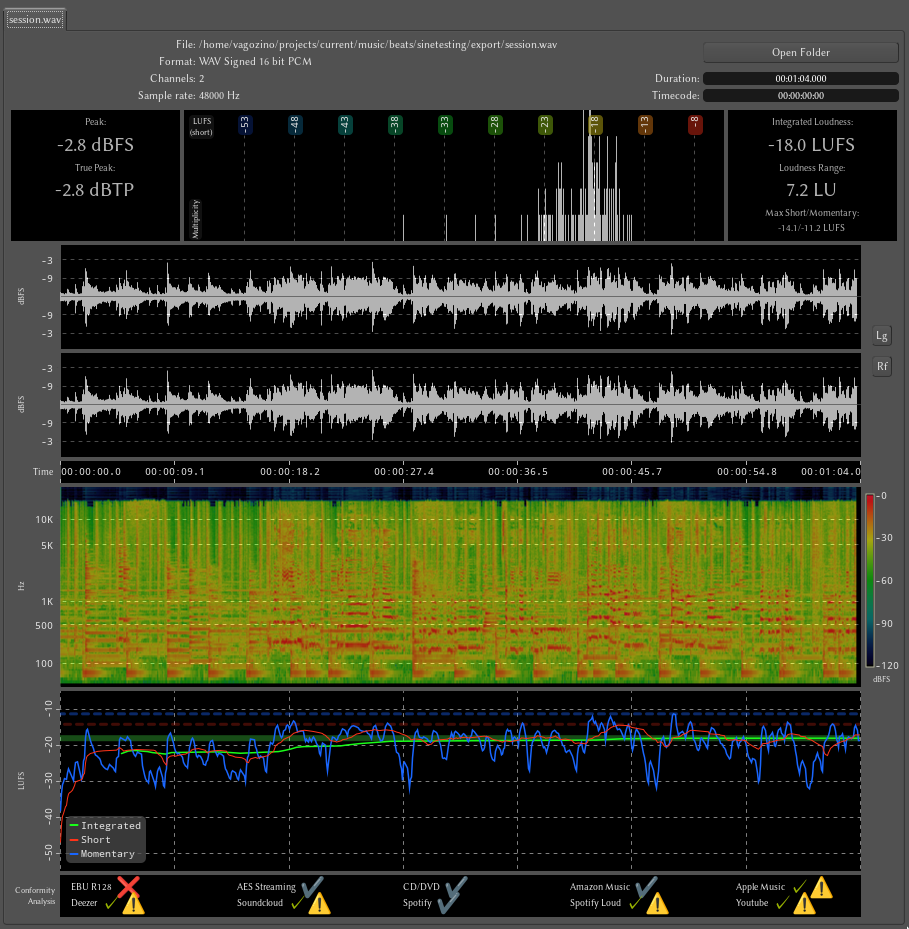
\includegraphics[width=0.5\textwidth]{./assets/session.png}
    \caption{Ανάλυση του αρχείο \src{BringMetTheDiscordKing.wav} χωρίς εφαρμογή του \en{plugin}.}
    \label{fig:sessionanalysis}
\end{figure}

\begin{figure}[htpb]
    \centering
    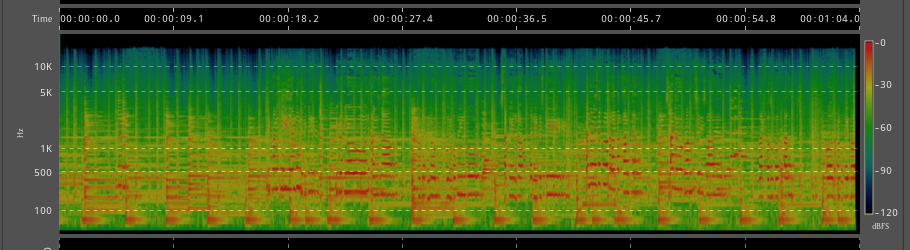
\includegraphics[width=0.5\textwidth]{./assets/session_1000_lp.png}
    \caption{Ανάλυση του αρχείο \src{BringMetTheDiscordKing.wav} με εφαρμογή χαμηλοπερατού φίλτρου στα $1000Hz$.}
    \label{fig:sessionanalysislp1000}
\end{figure}

\begin{figure}[htpb]
    \centering
    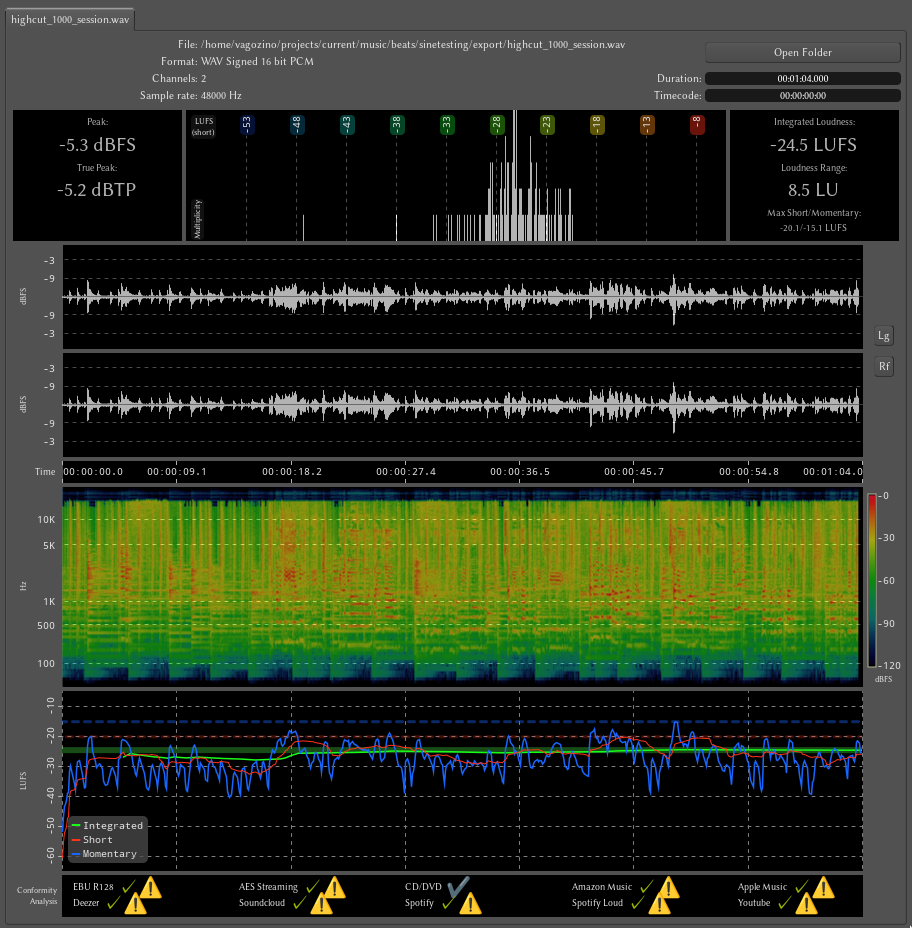
\includegraphics[width=0.5\textwidth]{./assets/session_1000_hp.png}
    \caption{Ανάλυση του αρχείο \src{BringMetTheDiscordKing.wav} με εφαρμογή υψιπερατού φίλτρου στα $1000Hz$.}
    \label{fig:sessionanalysishp1000}
\end{figure}


\newpage

\bibliography{bibliography}

\end{document}
